
\chapter{\label{cha:intro}Introduction}

As social networks are gaining more popularity today, the graph model is found to be a natural data model in numerous areas. For example, Figure \ref{fig:new-example} models a researcher network, in which nodes represent entities such as professors, papers, universities, etc., and edges are diverse relationships between them.
\\A graph database is a database that uses graph structures with nodes, edges and properties to store and query data. One problem of existing graph databases is that none of them support distributed storage and distributed evaluation of regular path query (RPQ) at the same time. So in this project, we investigate distributed algorithms on Apache HBase/Cassandra (Distributed Storage) and Apache Spark (Distributed Computation) to evaluate regular path query.

\begin{figure}[h!]
  \caption{Example - Researcher Network}
  \label{fig:new-example}
  \centering
    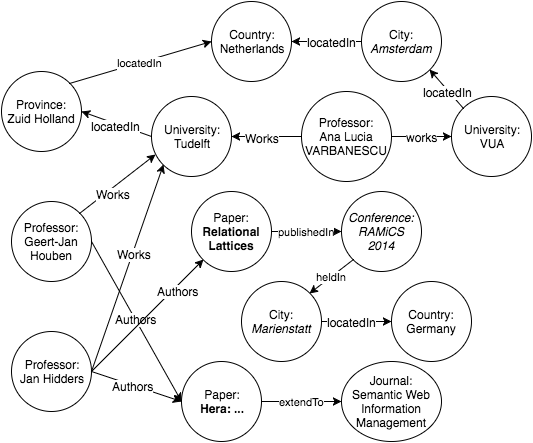
\includegraphics[width=0.5\textwidth]{img/new-example}
\end{figure}

A regular path query (RPQ) consists of node variables $X,Y$ and regular expression $R$ in the form of $(X,R,Y)$. The result should be pairs of nodes $(x,y)$ where there exists a path between them that the edge-label sequence of the edges satisfying $R$. For example, we can run several RPQs for Research Network in Figure \ref{fig:new-example}:
\begin{enumerate}
    \item $(X,authors*author^-,Y)$: Finding two professors who co-author a same paper. In this network, the result will be pairs (Jan Hidders, Geert-Jan Houben) and (Geert-Jan Houben, Jan Hidders), since there are paths between the nodes representing those two professors that satisfy the regular expression.
    \item $(X,works*locatedIn^*,Y)$: Finding all places where the professors work in, the result can be (Ana, VUA), (Ana, Zuid Holland), (Jan Hidders, Netherlands), etc. Here we introduce kleene star since the locations can be at different levels( university, city or country ).
    \item $(X,author*(publishedIn|extendTo))$: This query will return the pairs of professor and conference/journal.
\end{enumerate}
The usual way to evaluate RPQ is cascaded two-way join, multi-way join\cite{afrati2010optimizing}, and Dan Suciu proposed a distributed architecture/algorithm for RPQ evaluation\cite{suciu2002distributed}. In distributed computation context, network communication is usually a crucial overhead/bottleneck during computation. One observation of the experiments about Dan Suciu's algorithm is that different partition configurations for graphs will influence the size of data transmitted on the network. In this project, we will explore different properties of partition strategies for distributed graphs and their influence on communication cost for distributed RPQ evaluation algorithms.

\section{Research Questions}
The main goals of this thesis work can be divided into two parts, and they can be split into following sub-questions:
\begin{enumerate}
\item How to solve regular path queries and conjunctive regular path queries in parallel with Apache Spark?
    \begin{enumerate}
    % \item How to translate regular path queries into data structures we can evaluate with?
    \item What data model should be used for graph storage to evaluate regular path queries efficiently?
    \item How to implement distributed algorithms for efficient query evaluation with Apache Spark?
    \item What's the pros and cons for different algorithms?
    \end{enumerate}
\item How could different partition strategies optimize the querying performance?
\begin{enumerate}
    \item What is the crucial factors leading to the bottleneck? 
    \item How to improve those factors with different partitioning strategies in order to optimize the querying performance?
\end{enumerate}
% \item How to optimize the query performance for CRPQ with vertex signature tree (VS-tree) ?
%     \begin{enumerate}
%         \item How to use VS-tree to speedup query performance?
%         \item What's the trade-off between index size and speedup?
%     \end{enumerate}
\end{enumerate}

\section{Approach}
Firstly I will look for edge-labelled graph data-sets as the benchmark, and those containing data and queries at the same time or with various labels will be preferred. Secondly, the system which consists of Spark and Cassandra/HBase will be deployed. A suitable data model will be selected to store benchmark graphs. When coming to implementation, experiments will be conducted with different algorithms and increasing number of workers for RPQ. For Dan Suciu's algorithm, different partitioning strategies will be examined with regards to different graph properties, running time and network communication of applications.

\section{Outline}
In Chapter 2 we will explore the research background briefly, including existing graph databases, regular path queries and related algorithms. Chapter 3 presents the basic data model, system architecture and the benchmarks. In Chapter 4-6 we will focus on introducing and giving the execution process in Spark for different distributed algorithms. After that, those algorithms will be evaluated and compared in Chapter 7. In chapter 8 we investigate the reason different partition strategies affect performance and develop a new distributed partition strategy to minimize the number of $input-nodes$. Finally we will give conclusion in Chapter 9.